\documentclass[slovene,11pt,a4paper]{article}
%\usepackage{fullpage}
\usepackage[margin=2cm]{geometry}

\usepackage[T1]{fontenc}



%dodatni paketki:
\usepackage{braket} %paket za bra in ket
\usepackage{graphicx}
\usepackage{amsmath,amsfonts,amsthm} %matematicni paket
\usepackage{color} % omogoča barvno pisanje
\usepackage[utf8]
{inputenc}
\usepackage[slovene]{babel} % slovenski jezik/hyphenation
\usepackage{hyperref} %naredi vse povezave rečerenc, kazala,...
\numberwithin{equation}{section} % Number equations within sections (i.e. 1.1, 1.2, 2.1, 2.2 instead of 1, 2, 3, 4)
\numberwithin{figure}{section} % Number figures within sections (i.e. 1.1, 1.2, 2.1, 2.2 instead of 1, 2, 3, 4)
\numberwithin{table}{section} % Number tables within sections (i.e. 1.1, 1.2, 2.1, 2.2 instead of 1, 2, 3, 4)
\usepackage{eurosym} %za znak €

\usepackage{mathrsfs}
\usepackage{mathabx} % za kemisjke smeri in naslednje 3 vstrice
\catcode`_=12
\begingroup\lccode`~=`_\lowercase{\endgroup\let~\sb}
\mathcode`_="8000


\usepackage{placeins}

\usepackage[margin=2cm]{geometry}



\begin{document}
\begin{titlepage}

\newcommand{\HRule}{\rule{\linewidth}{0.5mm}} % Defines a new command for the horizontal lines, change thickness here

\center % Center everything on the page

%----------------------------------------------------------------------------------------
%	LOGO
%----------------------------------------------------------------------------------------

%\includegraphics{Logo}\\[1cm] % Include a department/university logo - this will require the graphicx package
 
%----------------------------------------------------------------------------------------

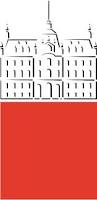
\includegraphics[width=2cm]{slike/aaa}\\[0.5cm]
 
%----------------------------------------------------------------------------------------
%	NASLOV DELA
%----------------------------------------------------------------------------------------
\textit{Univerza v Ljubljani}\\
\textit{Fakulteta za {\color{red}matematiko in fiziko}}\\[0.5cm]

\emph{Oddelek za fiziko}\\[0.5cm] % Oddelek za fiziko


%----------------------------------------------------------------------------------------
%	TITLE SECTION
%--------------------------------------------------------------------------------------
\HRule \\[0.4cm]
\huge {\bfseries Zaključna naloga}\\[0.4cm] % NASLOV SEMINARJA
\HRule \\[0.5cm] 

 \textsc{\large Poročilo pri predmetu modelska analiza 1}\\
 \textsc{\large 2015/2016}\\[1cm] % SEMINASKO DELO
 
%----------------------------------------------------------------------------------------
%	AUTHOR SECTION
%----------------------------------------------------------------------------------------



% If you don't want a supervisor, uncomment the two lines below and remove the section above
\Large \emph{Avtor:}\\
Klemen \textsc{Rahne}\\
28152028\\[2cm]
%----------------------------------------------------------------------------------------
%	DATUM
%----------------------------------------------------------------------------------------

{\large \today } \\[0.5cm] % Date, change the \today to a set date if you want to be precise

	

\end{titlepage}


%----------------------------------------------------------------------------------------
%	KAZALO
%----------------------------------------------------------------------------------------

%\tableofcontents

%----------------------------------------------------------------------------------------
%	ZAČETEK TEKSTA
%----------------------------------------------------------------------------------------


\section{Naloga}
Plastična kocka, v kateri se nevtroni tako sipljejo, kot tudi absorbirajo, je premazana s tanko plastjo, ki seva nevtrone. Določi porazdelitev absorbiranih nevtronov po volumnu kocke pri različnih vrednostih absorpcijskih parametrov.

\section{Teoretični uvod}

\subsection{Sipanje na jedru atoma} \label{sipanje-na-jedru}
V snovi se nevtroni v snovi sipljejo na jedrih atomov v snovi. Verjetnost za trk nevtrona na jedru je odvisna od velikosti nevtrona, velikosti jedra na katerem se trka in gostote jeder v snovi. Predpostavimo, da je prosta pot nevtrona do trka porazdeljena eksponentno z karakteristično razdaljo $\lambda_S$. Karakteristično razdaljo $\lambda_S$ bomo predpostavili iz teorije kinetičnega plina:
\begin{equation}
\lambda_S = \frac{1}{\sqrt{2} n \sigma}
\end{equation}
kjer je $n$ številska gostota jeder v materialu in $\sigma$ presek za trk, v tem primeru prečni presek jedra v snovi. Zgornjo enačbo lahko preoblikujemo v bolj pomenljivo obliko. Številsko gostoto lahko zapišemo $n=\frac{N}{V}=\frac{m N_A}{V M}=\frac{\rho N_A}{M}=\frac{\rho N_A}{A}$
kjer je:
\begin{itemize}
\item $\rho$ gostota snovi
\item $N_A=6.022 \times 10^{23}mol^{-1}$ Avogadrova konstanta
\item $M=A$ molekulska gostota snovi
\end{itemize}
Podobno lahko presek za trk zapišemo kot prečno površino jedra $\sigma=\pi R^2=\pi (A^{\frac{1}{3}}r_0)^2=\pi A^{\frac{2}{3}} r_0^2$, kjer smo radij jedra zapisali v odvisnosti od števila nukleonov v jedru ($A$):
\begin{itemize}
\item $R$ radij jedra
\item $r_0=1.25\times 10^{-15}m$ konstanta 
\item $A$ število nukleonov v jedru oz. masno število snovi
\end{itemize}
Tako se nam zgornja enačba poenostavi v obliko:
\begin{equation}
\lambda_S = \frac{1}{\sqrt{2} \rho N_A A^{- \frac{1}{3}} \pi r_0^2}
\end{equation}
V nalogi imamo sredico kocke iz plastike. Gostota plastike je približno $1\frac{g}{cm^3}$, ter je večinoma sestavljena iz ogljikovodikov. Predpostavimo, da je večina jeder ogljikovih jeder z masnim številom $A=12$. S temi pogoji dobimo povprečno prosto pot nevtrona v plastiki okoli $\frac{1}{2}m$.\\
Zanima nas še kam se bo odbil sipani nevtron. Zaradi večje teže jedra in vezanosti v polimerni molekuli bo jedro na katerem se nevtron sipa mirovalo. Najprej potrebujemo točko na površini jedra, kjer se bo nevtron sipal. V prečnem preseku je verjetnost sipanja enakomerno porazdeljena po prečnem preseku. Če prečni presek zapišemo v polarnih koordinatah sta $\rho$ in $\alpha$ porazdeljena:
\begin{equation}
\begin{aligned}
\rho= & \sqrt{\xi_1}  \\
\alpha = & 2 \pi \xi_2
\end{aligned}
\end{equation}
kjer sta $\xi_1$ in $\xi_2$ porazdeljena enakomerno med $0$ in $1$. Sedaj moramo točko iz preseka krogle projecirati na površino sfere. V sferičnih koordinatah projecirano točko zapišemo:
\begin{equation}
\label{porazdelitev-kot-sfera-trk}
\begin{aligned}
\tan(\phi)=& \frac{\rho \sin(\alpha)}{\sqrt{1-\rho^2}} \\
\cos(\theta) = & \rho \cos(\alpha)
\end{aligned}
\end{equation}

Preverimo, če je porazdelitev točk trkanja na jedrih enakomerna porazdeljena po preseku jedra.



\begin{figure}[!htb]
\centering
\begin{minipage}{0.5\textwidth}
\centering
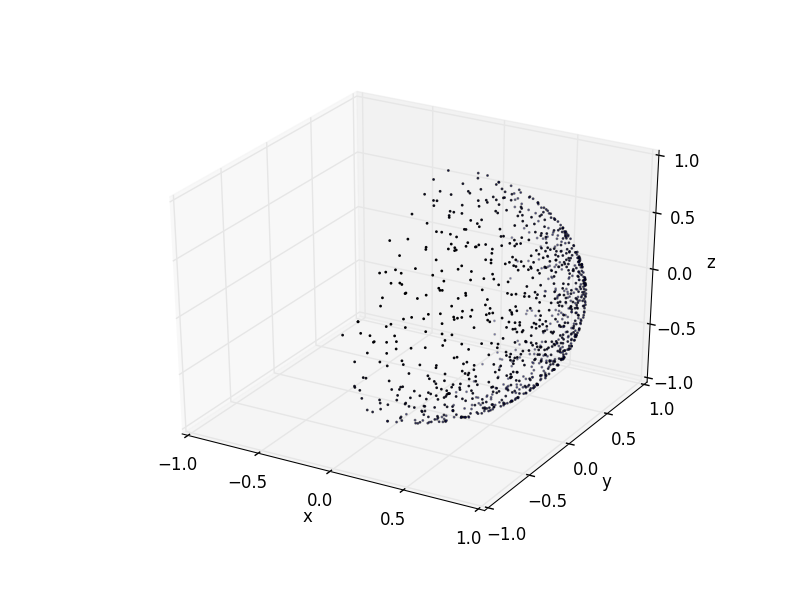
\includegraphics[scale=0.45]{slike/porazdelitev_tock_trka_na_jedru.png}
%\caption{first figure}
\end{minipage}\hfill
\begin{minipage}{0.5\textwidth}
\centering
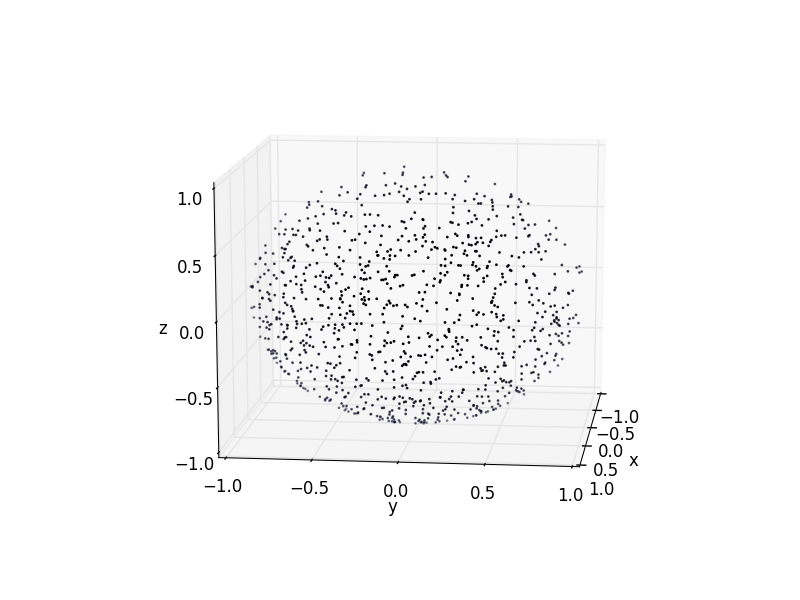
\includegraphics[scale=0.45]{slike/porazdelitev_tock_trka_na_jedru_1.png}
%\caption{second figure}
\end{minipage}

\caption{Porazdelitev točk trka na jedru. Na levem grafu vidimo, da so točke porazdeljene samo po desni polovici sfere. Iz tega lahko sklepamo, da je kot $\phi$ porazdeljen med $- \frac{\pi}{2}$ in $\frac{\pi}{2}$, medtem ko je kot $\theta$ porazdeljen med $0$ in $\pi$. Desni graf je enak levemu, le projekcija je druga (pogled iz osi $y$) in se lepo vidi enakomerna porazdelitev po preseku jedra.}
\end{figure}

\FloatBarrier

Zgoraj ponazorjena porazdelitev točk trka na jedru velja samo za trke, ko nanj trči nevtron v smeri osi $y$. Zato je potrebno porazdelitev zasukati, odvisno iz katere smeri nevtron prihaja. Predpostavimo, da nevtron prihaja v smeri $\theta'$ in $\phi'$. Ker je na sferi/jedru možen trk le na polovici katero nevtron vidi, je potrebno kota $\theta$ in $\phi$ (ki ju naključno izžrebamo po enačbi \ref{porazdelitev-kot-sfera-trk}) primerno zasukati:

\begin{equation}
\begin{aligned}
\theta_{nov}=& \theta + \theta' + \frac{\pi}{2} \\
\phi_{nov} = & \phi + \phi' + \pi
\end{aligned}
\end{equation}
Pri transformaciji kota $\theta$, je potrebno paziti, da je nov kot na intervalu med $0$ in $\pi$. V nasprotnem primeru, ko ima kot vrednost med $\pi$ ter $ 2 \pi$ nam točko na sferi/jedru preslika čez ravnino $xy$.  Temu se izognemo tako, da vzamemo od kota $\theta_{nov}$ modulo $2 \pi$. V primeru, ko je kot ta vrednost še vedno večja od $\pi$, kotu priredimo novo vrednost: $\theta_{nov}' = 2 \pi - (\theta_{nov}\mod 2 \pi ) $ .\\
Sedaj imamo točko trka na jedru/sferi in jo označimo $\vec{A}$. Ker poznamo  smer vpadnega nevtrona ($\vec{B}$) lahko določimo smer odbitega nevtrona ($\vec{C}$):
\begin{equation}
\vec{C}=\vec{B}+2 proj_{\vec{A}}\vec{B}
\end{equation}


\begin{figure}[!htb]
\centering
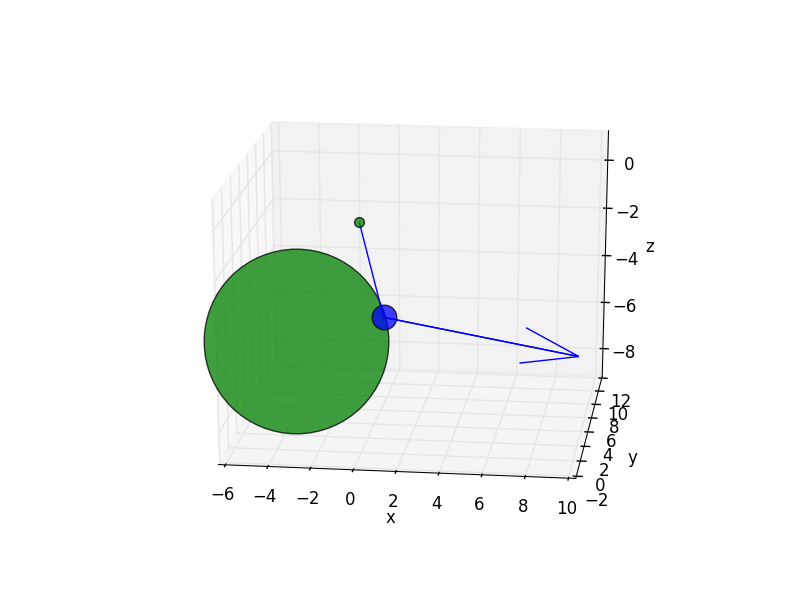
\includegraphics[scale=0.4]{slike/trk_na_jedru.png}
\caption{Grafična ponazoritev trka nevtrona ob jedro.}
\end{figure}


\subsection{Absorpcija nevtrona}

Obravnava absorpcije nevtrona v snovi je lažja kot sipanje nevtrona v snovi. Nevtron se lažje veže v jedro atoma, ker je nevtralno nabit, v primerjavi s protonom, za katerega je potrebna dodatna energija, ki premaga odbojno elektrostatsko energijo jedra. Ponavadi postane po absorpciji nevtrona jedra v vzbujenem stanju, ki se s pomočjo izseva gama žarkov pride v osnovno stanje. Podobno kot pri sipanju jedra je prosta pot nevtrona porazdeljena eksponentno z karakteristično razdaljo $\lambda$. Karakteristična razdalja je odvisna od preseka za absorpcijo $\sigma_A$, ki je med drugim odvisen od materiala in energije nevtrona.:


\begin{equation}
\lambda = \frac{1}{\sqrt{2} n \sigma_A} = \frac{1}{\sqrt{2} \rho \frac{N_A}{A} \sigma_A}
\end{equation}

Zaradi močne energijske odvisnosti preseka za absorpcijo nevtrona, bomo raziskali vrednosti $\lambda_A$ v območju velikostnega reda $\lambda_S$.

\section{Absorpcija nevtronov v kocki}

V prejšnjih poglavjih smo pogledali, kako se obnaša nevtron v snovi. Oglejmo si porazdelitev absorpcije nevtronov v kocki. Zaradi simetričnosti kocke v vseh treh dimenzijah, bomo porazdelitev absorpcije nevtronov gledali le v sredinskem preseku. Pri našem modelu imamo na površini kocke tanko plast nevtronskih sevalcev. Pri simulaciji, bomo nevtrone enakomerno porazdelili na vsako stranico kocke. Nato bomo vsakemu nevtronu določili naključno smer:
\begin{equation}
\begin{aligned}
\phi &= 2 \pi \xi_1 \\
\theta &=\arccos( 2 \xi_2 -1)
\end{aligned}
\end{equation}
kjer sta $\xi_1$ in $\xi_2$ porazdeljena enakomerno. Prav tako vsakemu nevtronu priredimo razdaljo v kateri se bo absorbiral v kocki. Ker je absorpcija statistični pojav, kjer je razdalja porazdeljena eksponentno ter odvisna od povprečne proste poti $\lambda$. Torej vsakemu nevtronu priredimo razdaljo:
\begin{equation}
r=- \lambda \log(1-\xi)
\end{equation}
kjer je $\xi$ ponovno porazdeljen enakomerno.
Sedaj imamo smer in razdaljo, ki jo potreboval do točke absorpcije. Iz začetnega položaja nevtrona sedaj preverimo ali je točka absorpcije v kocki.\\
V primeru, da upoštevamo še sipanje, je potrebno pri določitvi smeri in poti do absorpcije nevtrona še določiti razdaljo do sipanja nevtrona na jedru materialna iz katere je kocka. Ponovno bomo to obravnavali statistično in privzeli eksponentno porazdelitev z parametrom povprečne proste poti za sipanje $\lambda_S$:
\begin{equation}
r_S=\lambda \log(1-\xi)
\end{equation}
kjer je $\xi$ ponovno enakomerno porazdeljena spremenljivka. Sedaj moramo še preveriti, ali se zgodi prej absorpcija ali sipanje (primerjamo generirani razdalji). V primeru, da se prej zgodi sipanje nevtronu spremenimo smer, kot opisano v poglavju \ref{sipanje-na-jedru}. Nato ponovno generiramo novo razdaljo do sipanja in primerjamo ali se prej zgodi sipanje ali absorpcija. Ta postopek ponavljamo dokler se nevtron ne absorbira ali pa odleti iz naše kocke.







\begin{figure}[!htb]
\centering
\begin{minipage}{0.5\textwidth}
\centering
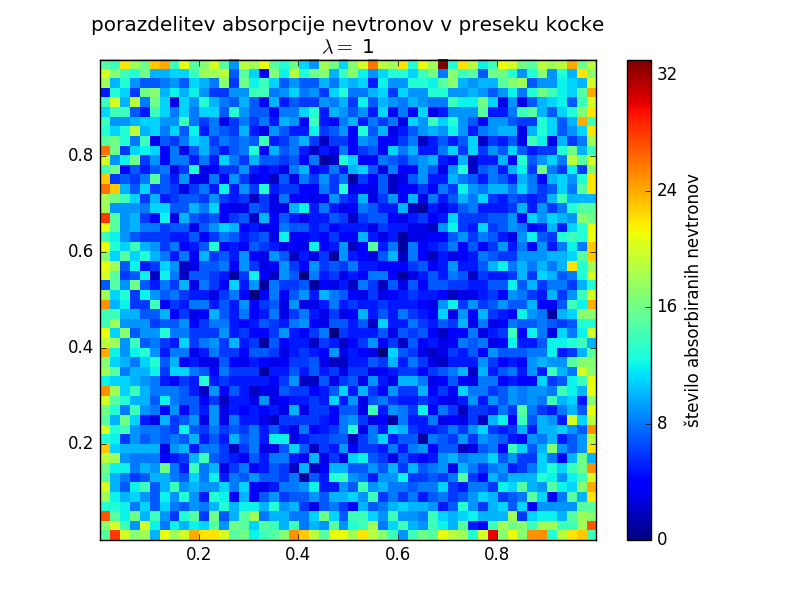
\includegraphics[scale=0.45]{slike/porazdelitev_lamda_1n_100000.png}
%\caption{first figure}
\end{minipage}\hfill
\begin{minipage}{0.5\textwidth}
\centering
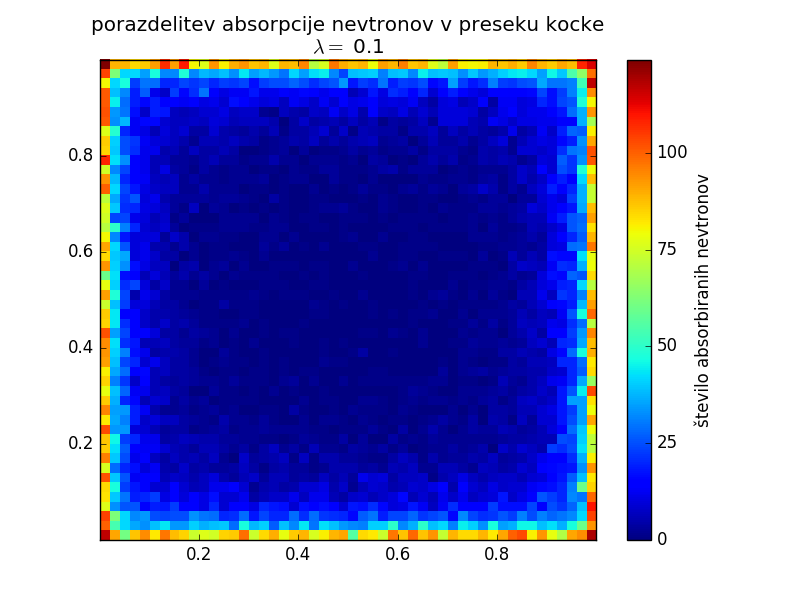
\includegraphics[scale=0.45]{slike/porazdelitev_lamda_0_1n_100000.png}
%\caption{second figure}
\end{minipage}
\caption{ Porazdelitev absorpcije nevtronov v preseku kocke. V tem primeru smo obravnavali samo absorpcijo, brez sipanja nevtronov. Na vsaki površini smo generirali $10^5$ nevtronov. Povsem pričakovano vidimo, da se največ nevtronov absorbira tik ob površini kocke. Razlika, ki je opazna v udorni globini, do kam pride največ nevtronov. Pri manjši prosti poti je pas, kjer se je absorbirala večina nevtronov ožji. Je pa v tem pasu tudi večja gostota absorbiranih nevtronov.}
\end{figure}



\begin{figure}[!htb]
\centering
\begin{minipage}{0.5\textwidth}
\centering
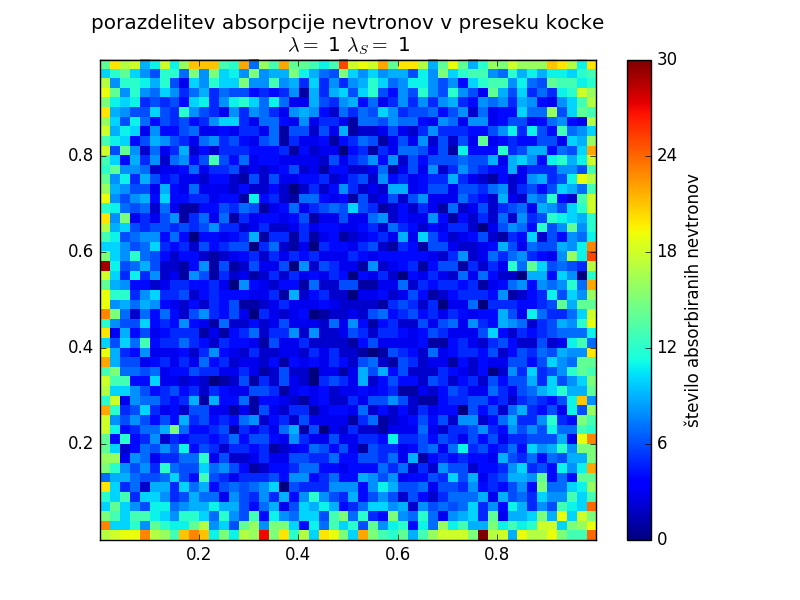
\includegraphics[scale=0.45]{slike/porazdelitev_lambda_s_1lamda_1n_100000.png}
%\caption{first figure}
\end{minipage}\hfill
\begin{minipage}{0.5\textwidth}
\centering
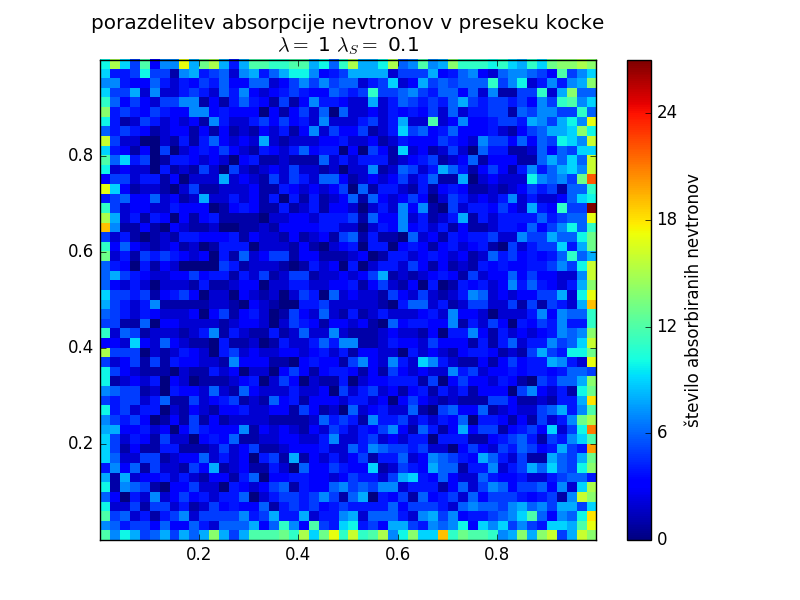
\includegraphics[scale=0.45]{slike/porazdelitev_lambda_s_0_1lamda_1n_100000.png}
%\caption{second figure}
\end{minipage}
\caption{Porazdelitev absorpcije nevtronov v preseku kocke z upoštevanjem sipanja nevtronov na jedrih. Pri krajši povprečni poti do sipanja, se nevtron večkrat siplje. Posledično se smer gibanja nevtrona večkrat spremeni in nimamo več lepo vidne prečne odvisnosti.}
\end{figure}







\begin{figure}[!t]
\centering
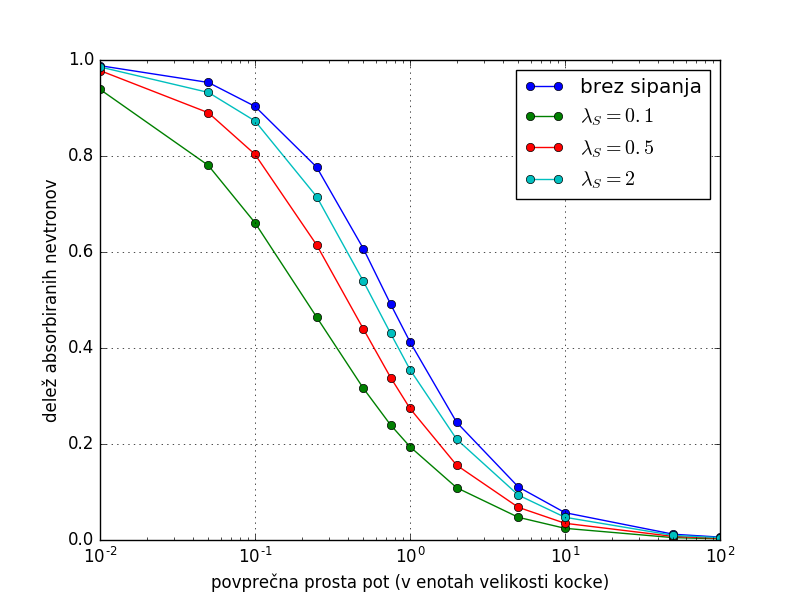
\includegraphics[scale=0.7]{slike/delez_absorbiranih_nevtronov.png}
\caption{Graf, ki ponazarja kako se spreminja delež absorbiranih nevtronov v odvisnosti od povprečne proste poti (v enoti dolžine stranice kocke). Opazimo, da v primeru večje proste poti delež nevtronov, ki se absorbirajo pada-kot da nevtroni materiala ne vidijo. Če upoštevamo še sipanje, se z krajšo prosto potjo sipanja delež absorbiranih nevtronov manjša. To je vzrok tega, da se pri krajših razdaljah nevtroni bolj sipljejo in nekaj nevtronov se siplje tako, da odletijo iz kocke. }
\end{figure}

\FloatBarrier

%-----------------------------------------------------------------------------------------------------------







%---------------------------------------------------------------------------------------------------------


\end{document}
